\documentclass[12pt,a4paper]{article}

\usepackage{latexsym}
\usepackage{url}
\usepackage{xspace}
\usepackage{epsfig}
%\usepackage{psfrag}
\usepackage{marvosym}
\usepackage{amsmath,amsfonts,amssymb,amsthm,latexsym}
\usepackage{graphics,graphicx,color,}
\usepackage{fancyhdr}
\usepackage{cite}
\usepackage[ngerman]{babel}
\usepackage[utf8]{inputenc}
\usepackage[T1]{fontenc}
%\textheight 680pt
%\textwidth 460pt
%\topmargin -40pt
%\oddsidemargin 5pt
%\evensidemargin 5pt
%\parindent 0pt

%\pagestyle{fancyplain} \setlength{\headheight}{16pt}
%\renewcommand{\sectionmark}[1]{\markright{\thesection\ #1}}
%\lhead[\fancyplain{}{\thepage}]
%    {\fancyplain{}{\rightmark}}
%\rhead[\fancyplain{}{\leftmark}]
%    {\fancyplain{}{\thepage}}
%\cfoot{}
%\renewcommand{\thesection}{\arabic{section}}
%\renewcommand{\thesubsection}{\arabic{section}.\arabic{subsection}}


\begin{document}
\begin{titlepage}%Institution
\vspace{2cm}
\centerline{
\large{Department of Computer Sciences}}
\vspace{0.2cm}
\centerline{\large{University of Salzburg}}%Title with one or two Lines(More if wanted)
%\hline
\vspace{2cm}

\centerline{\large{PS Software Praktikum}}
\centerline{WS 17/18}
\vspace{1cm}

\centerline{\Large{\bf{Cool Roofs}} }%Type of the Document
\vspace{1cm}

\vspace{0.4cm}%Date
\centerline{\today}
\vspace{5cm}%Authors

\vspace{0.2cm}
Project Members:
\begin{center}
  \begin{tabular}{rcl}
    Michael Nening,  & irgendwas,  & michael.nening@stud.sbg.ac.at \\
    Martin Schönegger,     & irgendwas,  & martin.schoenegger@stud.sbg.ac.at \\
    Timo Niederleuthner,& 01521540,  & timo.niederleuthner@stud.sbg.ac.at \\
    Michael Moser,    & irgendwas,  & michael.moser@stud.sbg.ac.at \\
  \end{tabular}
\end{center}
\vspace {1cm}


Correspondence to: \\
\centerline{Universit\"{a}t Salzburg} \\
\centerline{Fachbereich Computerwissenschaften} \\
\centerline{Jakob--Haringer--Stra\ss e 2} \\
\centerline{A--5020 Salzburg} \\
\centerline{Austria}
\clearpage
\end{titlepage}

%Table of Content
% \setcounter{page}{1}
% \pagenumbering{Roman} %I,II,III... in the TOC
% \tableofcontents

\clearpage



%Table of Content
% \setcounter{page}{1}
% \pagenumbering{Roman} %I,II,III... in the TOC
% \tableofcontents

%\pagestyle{headings}
\pagenumbering{arabic}  %Better if TOC is variable (more than one page)
\setcounter{page}{1}
\tableofcontents 
\clearpage


\section{Kurzfassung}
Das Projekt Cool-Roofs ist im Umfang der Lehrveranstaltung Software Praktikum der Universität Salzburg entstanden. Die globale Erwärmung ist ein allgegenwärtiges Problem; mit diesem Projekt soll ein Beitrag dagegen geleistet werden. Es gibt eine spezielle Farbe mit der Dächer angestrichen werden können, damit diese einen Großteil der Sonnenstrahlung zurück reflektieren. Auf diese Weise lässt sich der Treibhauseffekt eindämmen.\\
Im Rahmen dieses Projekts entwickelten wir eine Webapplikation, mit der sich Hausbesitzer und Investoren in Verbindung setzen können.Ein Hausbesitzer kann sein Dach registrieren, und Investoren finanzieren mit ihrer gezahlten Summe das Streichen des Daches. Dieses hat auch für die Dachbesitzer einen positiven Effekt: Die Häuser wärmen sich bei viel Sonneneinstrahlung nicht mehr so auf wie früher, was in einem angenehmeren Wohnklima resultiert und dazu führt, dass Klimaanlagen weniger oft eingeschalten werden müssen. Jeder Investor/Hausbesitzer soll außerdem eine Anzeige des gesparten CO$_2$ und eine Google-Maps Ansicht des Hauses bekommen.



\section{Einleitung} 
Mittags an einem klaren Sommertag in den Vereinigten Staaten erhält eine flache (horizontale) Oberfläche etwa 1000 Watt Sonnenlicht pro Quadratmeter. Traditionelle dunkle Dächer absorbieren dieses Sonnenlicht stark und erhitzen sowohl das Gebäude als auch die umgebende Luft. Dies erhöht den Energieverbrauch in klimatisierten Gebäuden und macht nicht klimatisierte Gebäude weniger komfortabel. Heiße dunkle Dächer verschärfen auch die städtischen Wärmeinseln, indem sie die über das Dach strömende Luft erwärmen und durch die Wärmeabstrahlung in die Atmosphäre zur globalen Erwärmung beitragen.\\
In unserer Webapplikation ist es möglich, sich entweder als Hausbesitzer oder als Investor einzuloggen. Dies ist einfach über einen vorhandenen Facebook/Google -Account möglich oder über eine normale Registrierung. Pro Account ist es nur möglich, entweder Investor oder Hausbesitzer zu sein.\\
Als Hausbesitzer ist man in der Lage seine Häuser auf einer Google-Maps-Karte einzuzeichnen. Gleichzeitig ist die Angabe von Dachtyp und Alter notwendig. Dabei wird die Fläche der Dächer automatisch über das gekennzeichnete Dach berechnet und muss nicht vom Hausbesitzer eingegeben werden. Außerdem sieht der Hausbesitzer, ob auf seinem Dach bereits eine Investition getätigt wurde und bekommt nach Anstrich des Daches eine Anzeige des gesparten C0$_2$.\\
Als Investor ist es nun möglich, sich ein Dach auszusuchen und in dieses zu investieren. Der Investor geht dafür auf die entsprechende Seite und kann dort die Region auswählen und wie viel m$^2$ er investieren möchte. Die Regionen sind dabei beschränkt auf Europe, Asia, North America, Africa, South America, Australia/Oceania, Other. Als nächstes werden ihm eine Reihe von verschiedenen Häusern vorgeschlagen, in welche er Investieren kann. Entweder bestätigt er diese oder er drückt auf Reset und bekommt eine neue Liste von Dächern angezeigt. Weiters hat der Investor Zugriff auf eine Ansicht all seiner Investitionen und sieht dabei das gesparte C0$^2$ pro Dach und in Summe und ein Google-Maps-Karte mit dem jeweiligen Dach.








\section{Verwendete Frameworks}
Im Projekt Cool-Roofs wurde mit Spring-Boot gearbeitet und damit verbunden mit diversen Frameworks. Hier werden wir Ihnen einen kurzen Überblick über die verwendeten Frameworks geben und anhand einiger Beispiele zeigen wie diese verwendet wurden.


\subsection{Spring-Boot MVC}
Das Spring-Boot MVC Framework stellt eine Model-View-Controller (MVC) Architektur und fertige Komponenten bereit, mit denen flexible und lose gekoppelte Webanwendungen entwickelt werden können. Das MVC-Muster führt zu einer Trennung der verschiedenen Aspekte der Anwendung, während eine lose Kopplung zwischen diesen Elementen bereitgestellt wird. 


\subsection{Maven}
Maven ist ein Build-Management-Tool der Apache Software Foundation und basiert auf Java. Dies hilft uns bei der Erstellung der ausführbaren .jar Datei.\\
In unserem Fall haben wir die Informationen für unser Softwareprojekt in ein XML-File mit dem Namen pom.xml gepackt. Diese Datei enthält alle Informationen zum Softwareprojekt. Auf den genaueren Aufbau wird noch eingegangen.


\subsection{Hibernate}
Hibernate ist ein ''Object-relational mapping'' (ORM) -Tool. Object-relational mapping oder ORM ist eine Programmiermethode zum Zuordnen der Objekte zum relationalen Modell, wobei Entitäten/Klassen Tabellen zugeordnet werde. Instanzen werden Zeilen zugeordnet und Attribute von Instanzen werden Tabellenspalten zugeordnet.\\
Es wird eine ''virtuelle Objektdatenbank'' erstellt, die innerhalb der Programmiersprache verwendet werden kann.\\
Näheres und Anwendungsbeispiele hierzu sind in der Beschreibung der Repositorys zu finden.


\subsection{Thymeleaf}
Thymeleaf ist eine moderne serverseitige Java-Template-Engine für Web- und Standalone-Umgebungen. Thymeleafs Hauptziel ist es, Templates in Ihren Entwicklungsworkflow zu bringen - HTML, das in Browsern korrekt dargestellt werden kann und auch als statischer Prototyp funktioniert, was eine stärkere Zusammenarbeit in Entwicklungsteams ermöglicht.\\
Mit Modulen für Spring Framework ist Thymeleaf ideal für unser Projekt in der HTML5 JVM-Webentwicklung. Mehr hierzu in den entsprechenden HTML-Dateien.


\subsection{Bootstrap}
Bootstrap ist ein Open-Source-Toolkit zur Entwicklung mit HTML, CSS und JS. Es enthält auf HTML und CSS basierende Vorlagen für Formulare, Buttons, Tabellen, Grid-Systeme, Navigations- und andere Gestaltungselemente. Bootstrap wird standardmäßig mit einem 940 Pixel breiten, zwölfspaltigen Grid-Layout ausgeliefert.\\
Wir verwendeten Bootstrap um unsere Website so zu gestalten, dass sie sowohl am PC wie auch am Smartphone/Tablet immer einwandfrei aussieht. 


\subsection{jQuery}
jQuery ist eine schnelle, kleine und funktionsreiche JavaScript-Bibliothek. Mit einer einfach zu verwendenden API, die für eine Vielzahl von Browsern geeignet ist. 
\clearpage




\section{Application Properties File}
Um unsere Anwendung lauffähig zu machen müssen vorerst einige Einstellungen vorgenommen werden.

\hspace{-5em}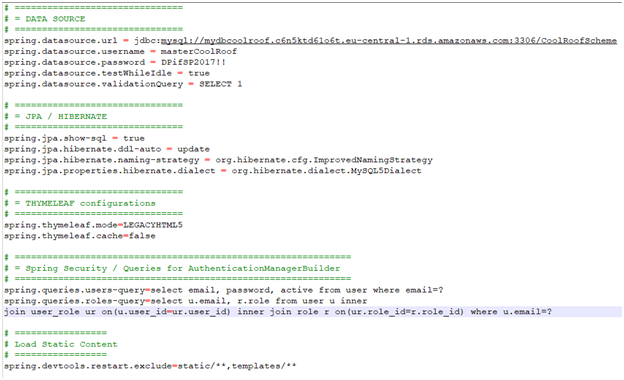
\includegraphics[width=1.2\textwidth]{./Graphics/bild1}

\begin{itemize}
	\item \textbf{Properties}\\
	Verschiedenste Eigenschaften können in der application.properties/application.yml Datei angegeben werden
	\item \textbf{Data Source}\\
	Hier wird die Datenquelle für unsere Web Applikation eingebunden. Für unsere Anwendung haben wir Amazon AWS als Datenbank verwendet. Wichtig hier ist die URL, den Usernamen und das Passwort der Datenbank bereitzustellen.
	\item \textbf{JPA / HIBERNATE}\\
	Der Befehl spring.jpa.show-sql = true wird verwendet um SQL Statements zu loggen. Die zweite Zeile spring.jpa.hibernate.ddl-auto = update wird verwendet, um die Datenbank bei Modelländerungen automatisch auf dem neuesten Stand zu halten. D.h. es werden automatisch Spalten in die Datenbank eingefügt, falls das Datenmodell verändert wird. Der dritte Befehl wird verwendet um Namen bei Datenbankanfragen automatisch mit ''\_'' zu versehen, was in Spring Boot bei einigen Datenbank Anfragen benötigt wird. Der vierte Befehl ermöglicht Hibernate, SQL zu generieren, welches für ein bestimmtes DBMS optimiert ist
	\item \textbf{Thymeleaf configurations}\\
	Hier ist es wichtig den Mode auf „LEGACYHTML5“ zu setzen um keine Probleme mit Thymeleaf in Kombination mit HTML5 zu bekommen.
	\item \textbf{Spring Security / Queries for AuthenticationManagerBuilder}\\
	Hier werden Queries für die Spring Security und den Authentication Manager Builder vordefinert.
	\item \textbf{Load Static Content}\\
	Diese Entwicklereinstellungen sind nützlich, um das Projekt in der Entwicklungsphase bei Änderung von statischem Inhalt nicht jedes Mal neu kompilieren zu müssen.
\end{itemize}


\subsection{Application.yml}

\hspace{-5em} 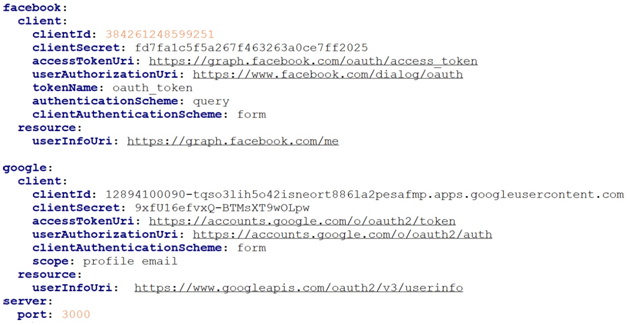
\includegraphics[width=1.2\textwidth]{./Graphics/bild2}

Diese Datei wird primär für unseren Social Media Login benötigt. Er beinhaltet diverse Einstellungen, welche von Facebook bzw. Google nach erfolgreicher Konfiguration zur Verfügung gestellt werden. Außerdem wurde hier der PORT festgelegt über welchen unsere Anwendung laufen soll.
\clearpage


\section{Project Object Model (POM) File}

\hspace{-5em} 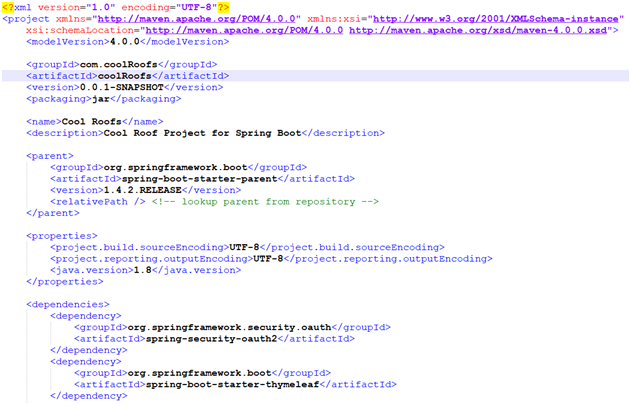
\includegraphics[width=1.2\textwidth]{./Graphics/bild3}

Ein Project Object Model oder POM ist die grundlegende Arbeitseinheit in Maven. Es ist eine XML-Datei, die Informationen über die Projekt- und Konfigurationsdetails enthält, die von Maven zum Erstellen des Projekts verwendet werden. Es enthält Standardwerte für die meisten Projekte.
Einige der Konfigurationen, die im POM angegeben werden können, sind die Projektabhängigkeiten, die Plugins oder Ziele, die ausgeführt werden können, die Erstellungsprofile und so weiter. Andere Informationen wie die Projektversion, Beschreibung, Entwickler, Mailinglisten und Ähnliches können ebenfalls angegeben werden.






\vspace{-10em} \section{SocialMediaController}\vspace{-1em}


\hspace{-5em} 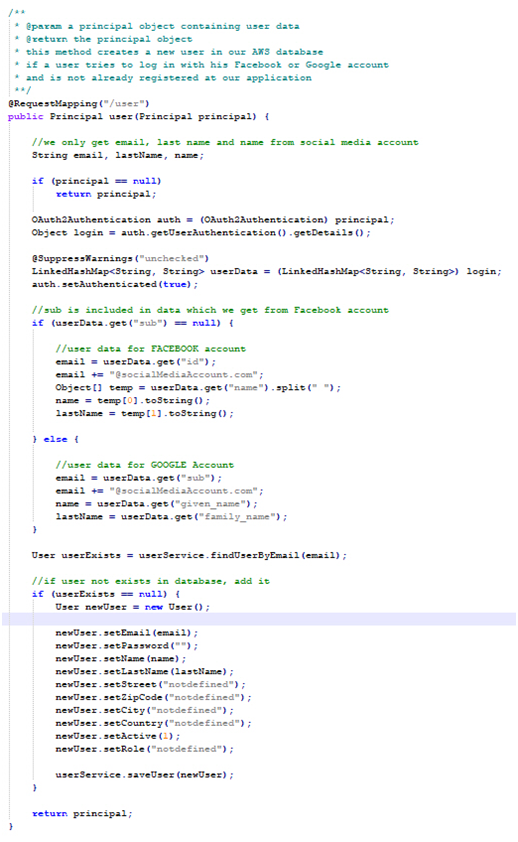
\includegraphics[width=1.1\textwidth]{./Graphics/bild4}

Dieser Controller verwaltet, wie der Name schon sagt, den Social Media Login. Er erhält im Prinzip vom Frontend ein Principal (represents the abstract notion of a principal, which can be used to represent any entity, such as an individual, a corporation, and a login id)  Objekt, welches von den sozialen Medien nach dem Login zur Verfügung gestellt wird.
Dieser Controller überprüft, ob sich der User zum ersten Mal auf unserer Seite einloggt oder ob er bereits in der Datenbank vorhanden ist.
Es gibt zwei Optionen welche erfüllt werden:

\begin{enumerate}
	\item Speichern des Users in die Datenbank und Rückgabe des User Objektes
	\item     Rückgabe des User Objektes, falls schon in Datenbank vorhanden
\end{enumerate}



\section{LoginController} 
Dieser Controller verwaltet den normalen (nicht social media) Login und die Registrierung von Nutzern. Im Prinzip legt der Nutzer über die Registration Page einen Account an. Die Zugangsdaten, sowie Art des Kontos und die getätigten Investments werden in der Datenbank gespeichert und bei Zugriffen auf die Seite(Login) von der Datenbank abgefragt. 

\hspace{-5em} 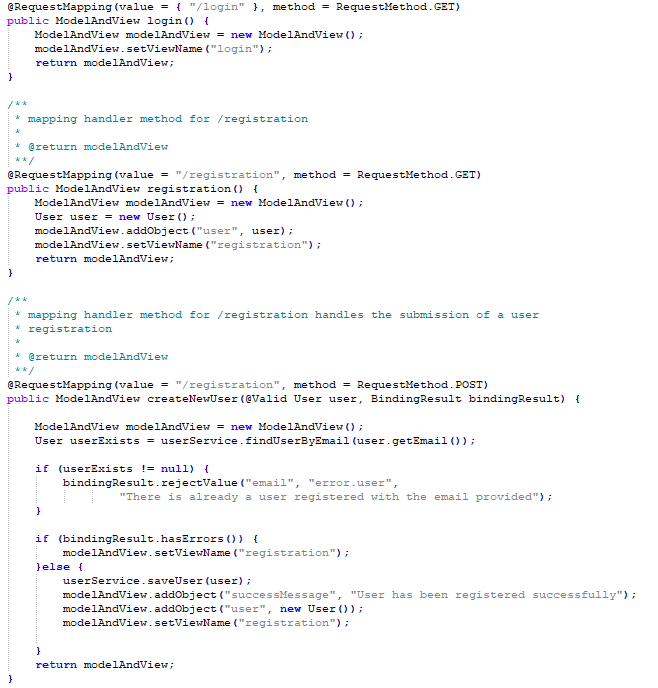
\includegraphics[width=1.2\textwidth]{./Graphics/bild5}

Als (eindeutigen) Benutzernamen wird die E-Mail Adresse des Nutzers verwendet. Das Passwort wird verschlüsselt in unserer Datenbank abgespeichert. Zusätzlich werden bei der Registrierung noch einige persönliche Informationen abgefragt.







\section{Grundprinzip ModelViewController (MVC)}
MVC ist ein bekanntes Programmierparadigma, bei dem zur besseren Aufteilung das Programm in 3 Programm-Komponenten geteilt wird.
\begin{itemize}
	\item das Modell (Model)\\
	Dient zur Speicherung bestimmter Daten, z.B. zur Speicherung von Teilen des aktuellen Zustands der Anwendung.
	\item die Darstellung des Modells (View)\\
	Eine Ansicht (View) kann eine beliebige Ausgabe von Informationen sein, z. B. ein Diagramm, und dient damit zur Visualisierung.
	\item die Beeinflussung des Modells (Controller)\\
	Der Controller akzeptiert Eingaben und konvertiert sie in Befehle für das Modell (Model) oder die Ansicht (View).
\end{itemize}
Das Modell ist verantwortlich für die Verwaltung der Daten der Anwendung. Es antwortet auf die Anfrage von der Ansicht und antwortet auch auf Anweisungen von der Steuerung, um sich selbst zu aktualisieren.\\
Die Ansicht bedeutet die Darstellung von Daten in einem bestimmten Format, ausgelöst durch die Entscheidung eines Controllers, die Daten zu präsentieren.\\
Der Controller ist dafür verantwortlich, auf die Benutzereingabe zu antworten und Interaktionen an den Datenmodellobjekten durchzuführen.





\section{MVC im Projekt}

Um das Model-View-Controller-Konzept einzusetzen, werden grob gesagt vier "Klassenarten"{} benötigt: Controller, Model, Repositoriy und Service. Im Folgenden Abschnitt wird auf die einzelnen Bestandteile näher eingegangen, mit je einer allgemeine Erklärung und einem kleinen Beispiel, wie das ganze in unserer Implementierung funktioniert.


\subsection{Controller}

Einerseits steuern die Controller-Klassen quasi den "Flow"{} der Anwendung, also welche Seiten wann angezeigt werden, andererseits kann hier auch die nötige Logik implementiert werden.

Eingesetzt wird dafür die \texttt{springframework}-API.

\bigskip
Ein einfaches Beispiel einer typischen Controller-Funktion:

\bigskip
\hspace{-1cm}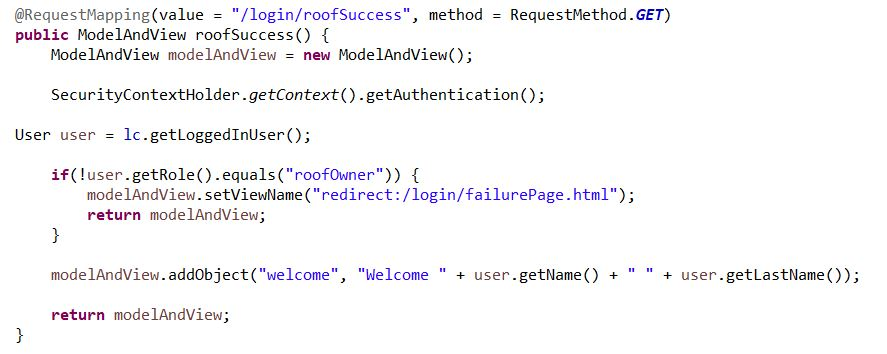
\includegraphics[scale=0.9]{./Graphics/controller_back}

\bigskip
Wann wird die Funktion aufgerufen? Dies wird über das \texttt{@RequestMapping} gesteuert. In diesem Fall also, wenn ein \texttt{GET} auf \texttt{/login/roofSuccess} angefragt wird.

\smallskip
Zuerst wird ein ModelAndView-Objekt erzeugt. Diesem können Informationen, die man anzeigen möchte, mitgegeben werden. In diesem einfachen Fall ist das der Name des Users, typischerweise sind das aber auch Model-Objekte, auf deren Attribute dann zugegriffen werden kann (via javascript und thymeleaf) oder die bei einer POST-Anfrage verändert werden können.

\smallskip
Zuvor überprüfen wir noch, ob der Nutzer eingeloggt ist und die richtige Rolle hat, also ob er überhaupt berechtigt ist, die Seite zu sehen. Wenn er das nicht darf, wird er nach /login/failurePage.html weitergeleitet.

\bigskip
\bigskip
Mit \texttt{@AutoWired} kann der Controller auf die Datenbank zugreifen und die damit verbundenen Methoden, die im Repository definiert wurden, benutzen.

\bigskip
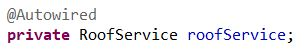
\includegraphics[width=0.5\textwidth]{./Graphics/autowired}

\bigskip
Das ganze wird als Attribut der Controller-Klasse definiert. Mehr Details zu den Repositories im dazugehörigen Kapitel.

\bigskip
\bigskip
Das dem ModelAndView-Objekt hinzugefügte Object kann dann im html file verwendet werden, in unserem Beipsiel einfach mit

\smallskip
\texttt{<div class="logged-in-user" th:utext= "\${welcome}"{}></div>}

\smallskip
Ein dem ModelAndView hinzugefügtes Roof-Objekt und dessen Felder kann am Frontend dann folgendermaßen verwendet werden:

\bigskip
\texttt{th:object="\${roof}"}

\bigskip
Und auf das "{}age"{} Feld des Roof-Objekts:

\bigskip
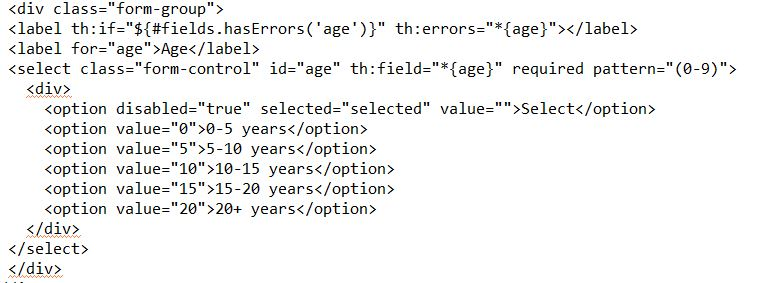
\includegraphics[scale=1]{./Graphics/controller_front}

\bigskip
\bigskip
Eine vollständige Controller-Klasse sollte natürlich für jede mögliche \texttt{GET}- und \texttt{POST}-Anfrage eine dazugehörige Funktion haben, die steuert, was bei der jeweiligen Anfrage dem Nutzer angezeigt werden soll.

\pagebreak


\subsection{Model}

Das Model stellt vereinfacht gesagt ein Objekt dar, dessen Attribute beispielsweise durch das Ausfüllen eines Formulars gesetzt werden können. Gleichzeitig werden diese Objekte auch zum Eintragen in die Datenbank genutzt.

\bigskip
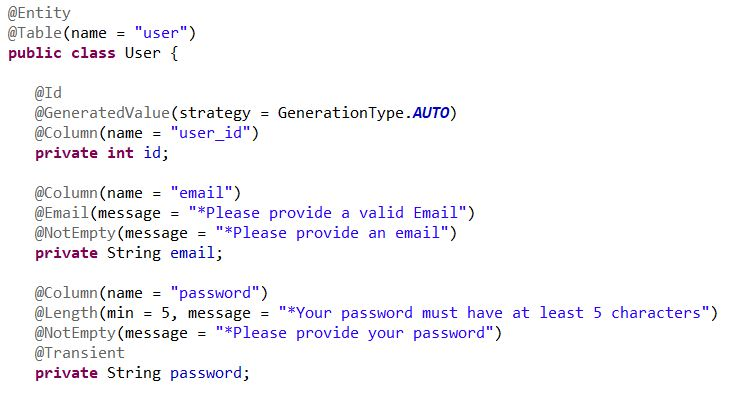
\includegraphics[width=1.1\textwidth]{./Graphics/model_back}

\bigskip
In diesem Beispiel definieren wir mit \texttt{@Table(name="{}user")}, dass ein User-Objekt einem Eintrag in unserer user-Tabelle der Datenbank entspricht. Selbiges natürlich mit \texttt{@Column} etc.

\smallskip
Diese Funktionalität wird von \texttt{javax.persistence.*}-API bereitgestellt. Eine weitere nützliche Funktion ist \texttt{@GeneratedValue(strategy = GenerationType.AUTO)}. Hier werden automatisch eindeutige Zahlen generiert, wie wir sie beispielsweise für die User-id verwenden. 

\bigskip
Zusätzlich findet man in der \texttt{hibernate.validator.constraints}-API einige sehr nützliche Funktionen:
\begin{itemize}
	\item \texttt{@Length} erlaubt, die Länge des Strings zu beschränken. So fangen wir zu kurze Passwörter ab.
	\item \texttt{@NotEmpty} stellt sicher, dass der übergebene String nicht leer ist.
	\item Mit \texttt{@Min(value)} kann festgesetzt werden, dass einem Integer (beispielsweise) nur Zahlen größer gleich \texttt{value} zugewiesen werden können.
	\item Weitere Funktionen: \texttt{@Email}, \texttt{@URL}, ...
\end{itemize}

\bigskip
Mit diesen Constraints kann man sehr einfach am Backend sicherstellen, dass nur erlaubte/gewünschte Werte in die Datenbank gelangen. 

\bigskip
Außerdem können direkt, wenn ein Input einen Constraint nicht erfüllt, Nachrichten übergeben werden, die dann beispielsweise der Nutzer sieht und erfährt, wo er einen Fehler gemacht hat. Zum Beispiel mit

\smallskip
\texttt{@Email(message="Please provide a valid Email")}.

\bigskip
Am Front-End wird das dann folgendermaßen ausgegeben:

\bigskip
\hspace{-2cm}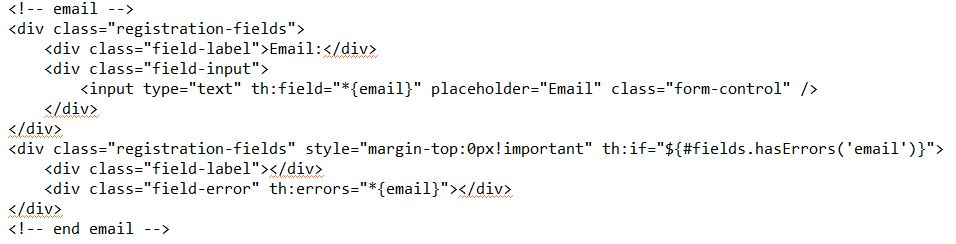
\includegraphics[scale=0.9]{./Graphics/model_front}

\bigskip
\bigskip
Ansonsten benötigt man in den Model-Klassen nur noch getter- und setter-Methoden.

\pagebreak


\subsection{Repository \& Service}

Mit den Repository-Interfaces wird JpaRepository erweitert. Die Repositories sind quasi die echte Schnittstelle zwischen Anwendung und Datenbank. Mit ihrer Hilfe werden die Queries erzeugt und beim Aufruf der entsprechenden Methode ausgeführt.

JpaRepositories stellt viele Teile von Datenbankabfragen bereit. Einige Beispiele sind hier aufgelistet:

\bigskip
\bigskip
\hspace{-3cm}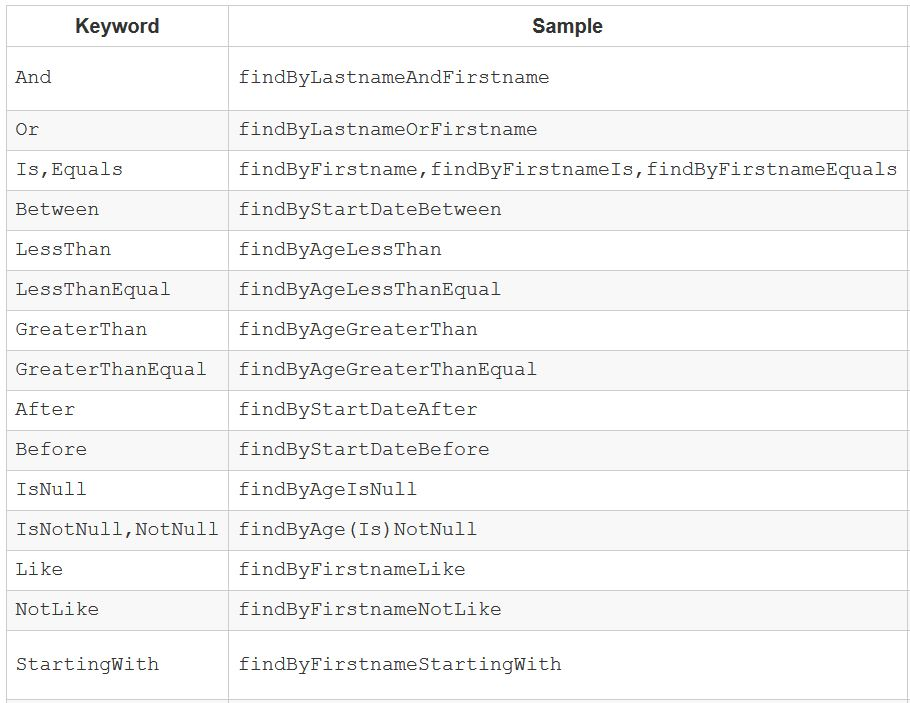
\includegraphics[scale=1]{./Graphics/jpa}
\url{https://docs.spring.io/spring-data/jpa/docs/1.5.0.RELEASE/reference/html/jpa.repositories.html} (Abschnitt 2.3.2)

\bigskip
\bigskip
Man kann sich damit die benötigten Methoden zusammenstellen, zum Beispiel im Format \texttt{find[All][Entity]By[Attribute]}.


\bigskip
\bigskip
Eine Beispiel aus unserem Projekt sind die drei Klassen RoofService + RoofServiceImplementation + RoofRepository.

\bigskip
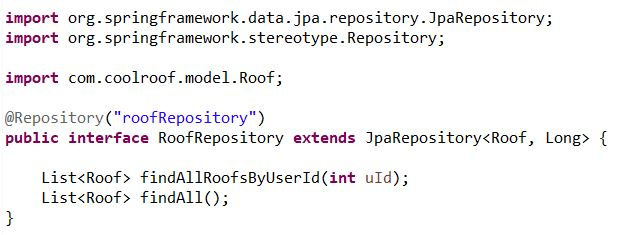
\includegraphics[scale=1]{./Graphics/repository}

\bigskip
Mit \texttt{@Repository} wird festgelegt, dass es ein Repository ist. Auf dieses kann, wie man beispielsweise in den Controllern sieht, über \texttt{@AutoWired} zugegriffen werden.

\bigskip
\bigskip
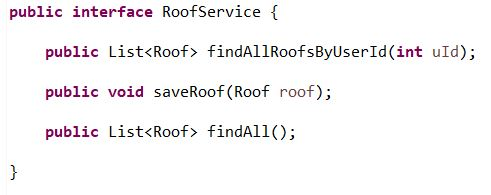
\includegraphics[scale=1]{./Graphics/service}

\bigskip
In diesem Interface werden die Methoden festgelegt, die dann in der RoofServiceImplementation implementiert werden.

\bigskip
\bigskip

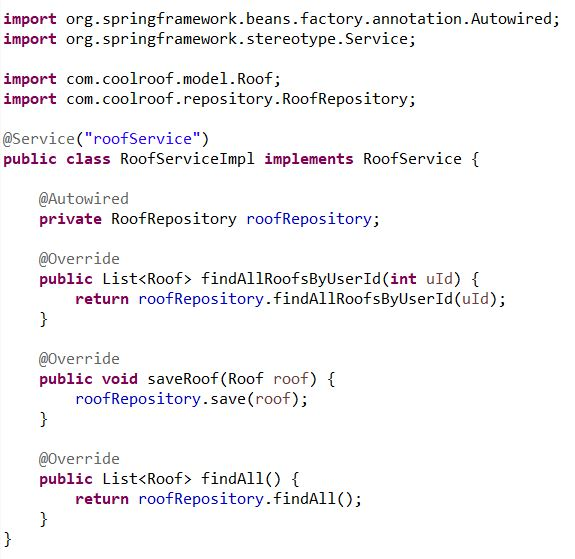
\includegraphics[scale=1]{./Graphics/service_impl}

\bigskip
Hier in der Implementierung ist schön zu sehen, wozu das Repository gut ist und wie man es benutzt. Da JpaRepository die Funktionen bereits bereitstellt, muss in der Implementation-Klasse nichts weiter getan werden als mit \texttt{@AutoWired} die Verbindung zum Repository herzustellen, und dann die passenden Funktionen aufzurufen. 

















% Exception Handling
\section{Exception Handling in Spring-Boot MVC}
Spring MVC bietet mehrere komplementäre Ansätze zum Exception Handling, hier werden wir nur kurz auf die wichtigsten Methoden eingehen um ein Grundverständnis zu erlangen.\\
Wir werden nun die verschiedenen verfügbaren Optionen zeigen. Unser Ziel ist es, Exceptions nicht explizit in Controller-Methoden zu behandeln, wo dies möglich ist. Sie werden besser in einem eigenen Code behandelt.\\
Die drei Optionen sind:
\begin{itemize}
	\item[\textbullet] per Exception
	\item[\textbullet] per Controller
	\item[\textbullet] oder global.
\end{itemize}


\subsection{HTTP Status Codes}
Normalerweise verursacht jede unbehandelte Ausnahme, die bei der Verarbeitung einer Webanforderung ausgelöst wird, dass der Server eine HTTP 500-Antwort zurückgibt. Jede Ausnahme, die man selbst schreibt, kann jedoch mit der Annotation @ResponseStatus versehen werden. Wenn eine mit Anmerkungen versehene Ausnahme von einer Controller-Methode ausgelöst wird und an keiner anderen Stelle behandelt wird, wird automatisch die entsprechende HTTP-Antwort mit dem angegebenen Statuscode zurückgegeben.


\subsection{Controller Based Exception Handling}
Man kann jedem Controller zusätzliche (@ExceptionHandler)-Methoden hinzufügen, um speziell Ausnahmen zu behandeln, die von Request-Handling-Methoden (@RequestMapping) im selben Controller ausgelöst werden. Solche Methoden könnten sein:
\begin{itemize}
	\item[\textbullet] Ausnahmen ohne die @ResponseStatus-Annotation (normalerweise vordefinierte Ausnahmen, die man nicht geschrieben hat) behandeln.
	\item[\textbullet] Den Benutzer in eine spezielle ''error view'' umleiten.
	\item[\textbullet] Eine vollständig benutzerdefinierte '' error response '' erstellen.
\end{itemize}


\subsection{Global Exception Handling}
Ein ''controller advice'' ermöglicht es, genau die gleichen Exception-Handling-Techniken zu verwenden, sie aber auf die gesamte Anwendung anzuwenden, nicht nur auf einen einzelnen Controller. Man kann sich diese als ''annotation driven interceptor'' vorstellen.\\
Jede mit @ControllerAdvice annotierte Klasse wird zu einem Controller-Advice und drei Arten von Methoden werden unterstützt:
\begin{itemize}
	\item[\textbullet] Exception-handling Methoden, die mit @ExceptionHandler kommentiert sind.
	\item[\textbullet] Model enhancement methods (zum Hinzufügen zusätzlicher Daten zum Modell), die mit @ModellAttribut kommentiert sind. Zu beachten ist dabei, dass diese Attribute für die ''exception handling views'' nicht verfügbar sind.
	\item[\textbullet] Binder-Initialisierungsmethoden (zur Konfiguration der Formularverarbeitung) mit  @InitBinder Anmerkungen versehen.
\end{itemize}



\section{Frontend Javascript}
JavaScript ist eine Skriptsprache, die ursprünglich 1995 von Netscape für dynamisches HTML in Webbrowsern entwickelt wurde, um Benutzerinteraktionen auszuwerten, Inhalte zu verändern, nachzuladen oder zu generieren und so die Möglichkeiten von HTML und CSS zu erweitern. Heute findet JavaScript auch außerhalb von Browsern Anwendung, so etwa auf Servern und in Microcontrollern.\\

Bei der Programmierung einer Webanwendung kommt man fast nicht um Javascript herum.
Der Javascript Code liegt in src/main/resources/static/javascript und ist in den Files ''make\_investment.js'', ''my\_investment'' und ''add\_roof.js''. (siehe Projekt Ordner)\\


Für das CoolRoof Projekt brauchen wir Javascript hauptsächlich für die Google Maps Integration, Kommunikation mit dem Backend und zum dynamischen Ändern des angezeigten Webinhaltes. \\


\hspace{-5em} 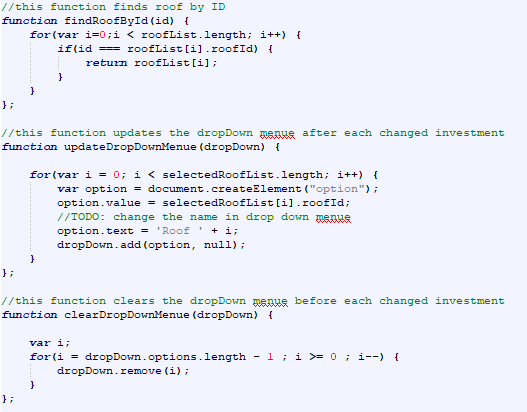
\includegraphics[width=1.2\textwidth]{./Graphics/bild6}\\


\noindent Funktionen um Dropdown-menüs Dynamisch zu verändern und eine Funktion um eine Liste aus Dächern zu durchsuchen. \\


\hspace{-5em} 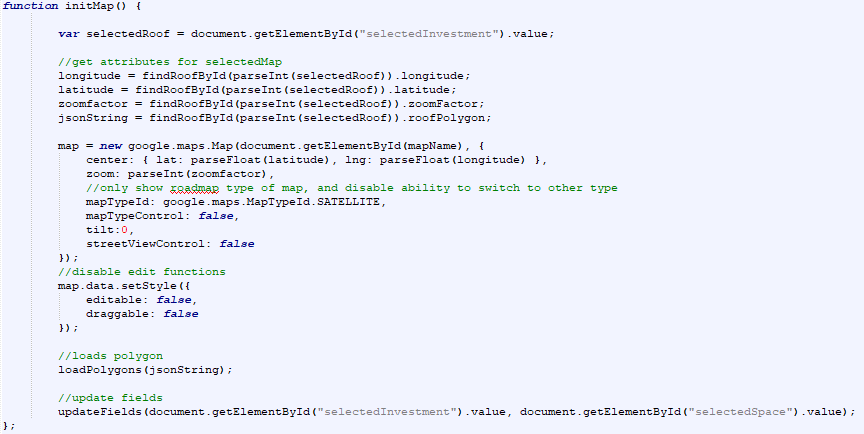
\includegraphics[width=1.2\textwidth]{./Graphics/bild7}\\

Google Maps Javascript Function






% Datenbank
\section{Datenbankmodel}
Als Anbieter für unsere Datenbank wählten wir AWS (AmazonWebServices). Hier gibt es spezielle Konten für Studenten, die es uns so möglich machten, alles zu benutzen was wir brauchten. Unser Datenbankmodell ist eine Relationale Datenbank, die MySQL unterstützt.


\subsection{RDS MySQL}
MySQL ist eine beliebte relationale Open-Source-Datenbank mit einfacher Skalierbarkeit.\\
Für die Organisation der Daten verwenden wir 5 verschiedene Tabellen. 
\begin{itemize}
	\item[\textbullet] Investment\\
	Beinhaltet Informationen über ein getätigtes Investment. (Fläche, Ort etc.)
	\item[\textbullet] Role\\
	Dient dazu um festzustellen, welche Rolle ein Benutzer hat.
	\item[\textbullet] Roof\\
	Beinhaltet Informationen über das Dach selbst. (Preis, Region etc.)
	\item[\textbullet] User\\
	Beinhaltet Informationen über den Benutzer. (Benutzername, Email etc.)
	\item[\textbullet] User\_Role\\
	Weist User ID einer Role ID zu.
\end{itemize}
Details hierzu sind in den jeweiligen Tabellen nachzusehen.\\

\textbullet Investment

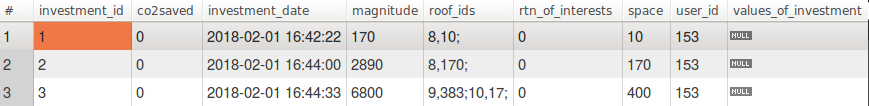
\includegraphics[scale=0.5]{./Graphics/investment}
\bigskip

\noindent \textbullet investemt\_id: Eindeutige ID vom Investment\\
\textbullet co2saved: Int Wert; wie viel CO$_2$ in Tonnen gespart wurde\\
\textbullet investment\_date: Datum, zu dem das Investment getätigt wurde\\
\textbullet magnitude: Wert des Investments in \$ \\
\textbullet roof\_id: Fremdschlüssel der Dächer \\
\textbullet space: Fläche in $m^2$\\
\textbullet user\_id: ID des Users\\
\bigskip

\textbullet Role

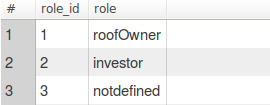
\includegraphics[scale=0.5]{./Graphics/role}

\noindent \textbullet role\_id: ID der Role\\
\textbullet role: Welche rolle der Account hat
\bigskip

\textbullet Roof

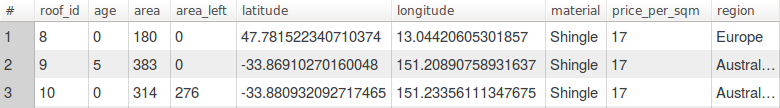
\includegraphics[scale=0.5]{./Graphics/roof1}

\noindent \textbullet roof\_id: ID des Daches\\
\textbullet age: Alter des Daches (0,5,10,15, >20 Jahre)\\
\textbullet area: Gesamtfläche des Daches\\
\textbullet area\_left: Fläche des Daches, in die noch nicht investiert wurde\\
\textbullet latitude: Breitengrad der Position des Daches\\
\textbullet longitud: Längengrad der Position des Daches\\
\textbullet material: Material des Daches\\
\textbullet price\_per\_sqm: Preis pro Quadratmeter in \$ \\
\textbullet region: Region, in der sich das Dach befindet\\
\bigskip

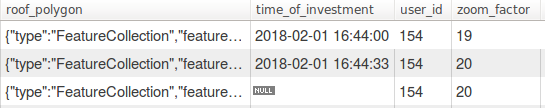
\includegraphics[scale=0.5]{./Graphics/roof2}

\noindent \textbullet roof\_polygon: Punkte des Daches in Form eines Strings\\
\textbullet time\_of\_investment: Datum, zu dem das Investment getätigt wurde\\
\textbullet user\_id: ID des Users\\
\textbullet zoom\_factor: Zoom Faktor für die Google-Maps Anzeige\\
\bigskip

\textbullet User

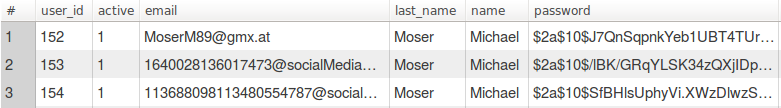
\includegraphics[scale=0.5]{./Graphics/user1}

\noindent \textbullet user\_id: ID des Users\\
\textbullet active: Ob noch aktuell \\
\textbullet emai: E-Mailadresse des Benutzers\\
\textbullet last\_name: Nachname des Benutzers\\
\textbullet name: Vorname des Benutzers\\
\textbullet password: Hashwert des Passwortes des Benutzers \\
\bigskip

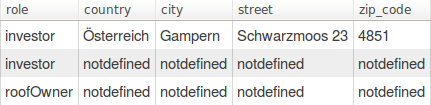
\includegraphics[scale=0.5]{./Graphics/user2}

\noindent \textbullet role: Rolle des Benutzers\\
\textbullet country: Land des Benutzers\\
\textbullet city: Stadt des Benutzers\\
\textbullet street: Straße des Benutzers\\
\textbullet zip-code: zip-code des Benutzers\\
\bigskip

\textbullet User\_Role

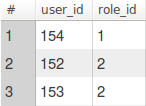
\includegraphics[scale=0.5]{./Graphics/user_role}

\noindent \textbullet user\_id ID des Benutzers\\
\textbullet role\_id: Rolle des Benutzers\\
\bigskip













\end{document}
